
\documentclass[11pt,compress,t,notes=noshow, xcolor=table]{beamer}
\usepackage[]{graphicx}\usepackage[]{color}
% maxwidth is the original width if it is less than linewidth
% otherwise use linewidth (to make sure the graphics do not exceed the margin)
\makeatletter
\def\maxwidth{ %
  \ifdim\Gin@nat@width>\linewidth
    \linewidth
  \else
    \Gin@nat@width
  \fi
}
\makeatother

\definecolor{fgcolor}{rgb}{0.345, 0.345, 0.345}
\newcommand{\hlnum}[1]{\textcolor[rgb]{0.686,0.059,0.569}{#1}}%
\newcommand{\hlstr}[1]{\textcolor[rgb]{0.192,0.494,0.8}{#1}}%
\newcommand{\hlcom}[1]{\textcolor[rgb]{0.678,0.584,0.686}{\textit{#1}}}%
\newcommand{\hlopt}[1]{\textcolor[rgb]{0,0,0}{#1}}%
\newcommand{\hlstd}[1]{\textcolor[rgb]{0.345,0.345,0.345}{#1}}%
\newcommand{\hlkwa}[1]{\textcolor[rgb]{0.161,0.373,0.58}{\textbf{#1}}}%
\newcommand{\hlkwb}[1]{\textcolor[rgb]{0.69,0.353,0.396}{#1}}%
\newcommand{\hlkwc}[1]{\textcolor[rgb]{0.333,0.667,0.333}{#1}}%
\newcommand{\hlkwd}[1]{\textcolor[rgb]{0.737,0.353,0.396}{\textbf{#1}}}%
\let\hlipl\hlkwb

\usepackage{framed}
\makeatletter
\newenvironment{kframe}{%
 \def\at@end@of@kframe{}%
 \ifinner\ifhmode%
  \def\at@end@of@kframe{\end{minipage}}%
  \begin{minipage}{\columnwidth}%
 \fi\fi%
 \def\FrameCommand##1{\hskip\@totalleftmargin \hskip-\fboxsep
 \colorbox{shadecolor}{##1}\hskip-\fboxsep
     % There is no \\@totalrightmargin, so:
     \hskip-\linewidth \hskip-\@totalleftmargin \hskip\columnwidth}%
 \MakeFramed {\advance\hsize-\width
   \@totalleftmargin\z@ \linewidth\hsize
   \@setminipage}}%
 {\par\unskip\endMakeFramed%
 \at@end@of@kframe}
\makeatother

\definecolor{shadecolor}{rgb}{.97, .97, .97}
\definecolor{messagecolor}{rgb}{0, 0, 0}
\definecolor{warningcolor}{rgb}{1, 0, 1}
\definecolor{errorcolor}{rgb}{1, 0, 0}
\newenvironment{knitrout}{}{} % an empty environment to be redefined in TeX

\usepackage{alltt}
\newcommand{\SweaveOpts}[1]{}  % do not interfere with LaTeX
\newcommand{\SweaveInput}[1]{} % because they are not real TeX commands
\newcommand{\Sexpr}[1]{}       % will only be parsed by R
\newcommand{\xmark}{\ding{55}}%


\usepackage[english]{babel}
\usepackage[utf8]{inputenc}

\usepackage{dsfont}
\usepackage{verbatim}
\usepackage{amsmath}
\usepackage{amsfonts}
\usepackage{amssymb}
\usepackage{bm}
\usepackage{csquotes}
\usepackage{multirow}
\usepackage{longtable}
\usepackage{booktabs}
\usepackage{enumerate}
\usepackage[absolute,overlay]{textpos}
\usepackage{psfrag}
\usepackage{algorithm}
\usepackage{algpseudocode}
\usepackage{eqnarray}
\usepackage{arydshln}
\usepackage{tabularx}
\usepackage{placeins}
\usepackage{tikz}
\usepackage{setspace}
\usepackage{colortbl}
\usepackage{mathtools}
\usepackage{wrapfig}
\usepackage{bm}
\usepackage{amsmath}
\usepackage{pifont}
\usepackage{xcolor} %colored math symbols

\usetikzlibrary{shapes,arrows,automata,positioning,calc,chains,trees, shadows}
\tikzset{
  %Define standard arrow tip
  >=stealth',
  %Define style for boxes
  punkt/.style={
    rectangle,
    rounded corners,
    draw=black, very thick,
    text width=6.5em,
    minimum height=2em,
    text centered},
  % Define arrow style
  pil/.style={
    ->,
    thick,
    shorten <=2pt,
    shorten >=2pt,}
}

\usepackage{subfig}

% Defines macros and environments
\usepackage{../../style/lmu-lecture}


\let\code=\texttt
\let\proglang=\textsf

\setkeys{Gin}{width=0.9\textwidth}

\setbeamertemplate{frametitle}{\expandafter\uppercase\expandafter\insertframetitle}

\usepackage{bbm}
% basic latex stuff
\newcommand{\pkg}[1]{{\fontseries{b}\selectfont #1}} %fontstyle for R packages
\newcommand{\lz}{\vspace{0.5cm}} %vertical space
\newcommand{\dlz}{\vspace{1cm}} %double vertical space
\newcommand{\oneliner}[1] % Oneliner for important statements
{\begin{block}{}\begin{center}\begin{Large}#1\end{Large}\end{center}\end{block}}


%new environments
\newenvironment{vbframe}  %frame with breaks and verbatim
{
 \begin{frame}[containsverbatim,allowframebreaks]
}
{
\end{frame}
}

\newenvironment{vframe}  %frame with verbatim without breaks (to avoid numbering one slided frames)
{
 \begin{frame}[containsverbatim]
}
{
\end{frame}
}

\newenvironment{blocki}[1]   % itemize block
{
 \begin{block}{#1}\begin{itemize}
}
{
\end{itemize}\end{block}
}

\newenvironment{fragileframe}[2]{  %fragile frame with framebreaks
\begin{frame}[allowframebreaks, fragile, environment = fragileframe]
\frametitle{#1}
#2}
{\end{frame}}


\newcommand{\myframe}[2]{  %short for frame with framebreaks
\begin{frame}[allowframebreaks]
\frametitle{#1}
#2
\end{frame}}

\newcommand{\remark}[1]{
  \textbf{Remark:} #1
}


\newenvironment{deleteframe}
{
\begingroup
\usebackgroundtemplate{
\includegraphics[width=\paperwidth,height=\paperheight]{../style/color/red.png}}
 \begin{frame}
}
{
\end{frame}
\endgroup
}
\newenvironment{simplifyframe}
{
\begingroup
\usebackgroundtemplate{
\includegraphics[width=\paperwidth,height=\paperheight]{../style/color/yellow.png}}
 \begin{frame}
}
{
\end{frame}
\endgroup
}\newenvironment{draftframe}
{
\begingroup
\usebackgroundtemplate{
\includegraphics[width=\paperwidth,height=\paperheight]{../style/color/green.jpg}}
 \begin{frame}
}
{
\end{frame}
\endgroup
}
% https://tex.stackexchange.com/a/261480: textcolor that works in mathmode
\makeatletter
\renewcommand*{\@textcolor}[3]{%
  \protect\leavevmode
  \begingroup
    \color#1{#2}#3%
  \endgroup
}
\makeatother


\input{../../latex-math/basic-math}
\input{../../latex-math/basic-ml}
\input{../../latex-math/ml-nn}

\newcommand{\titlefigure}{figure/dilatedconv-7.png}
%modify picture
\newcommand{\learninggoals}{
  \item Dilated Convolutions
  \item Transposed Convolutions
}

\title{Deep Learning}
\date{}



\begin{document}

\lecturechapter{Important Types of Convolutions}
\lecture{I2DL}

%%%%%%%%%%%%%%%%%%%%%%%%%%%%%%%%%%%%%%%%

%%%%%%%%%%%%%%%%%%%%%%%%%%%%%%%%%%%%%%%%

%%%%%%%%%%%%%%%%%%%%%%%%%%%%%%%%%%%%%%%%%%%%%

\section{Dilated Convolutions}

\begin{vbframe}{Dilated convolutions}

    \begin{itemize}
        \item Idea : artificially increase the receptive field of the net without using more filter weights.
        \item The \textbf{receptive field} of a single neuron comprises all inputs that have an impact on this neuron. 
        \item Neurons in the first layers capture less information of the input, while neurons in the last layers have huge receptive fields and can capture a lot more global information from the input. 
        \item The size of the receptive fields depends on the filter size. 
    \end{itemize}

    \vspace*{-0.5cm}

    \begin{figure}
        \centering
        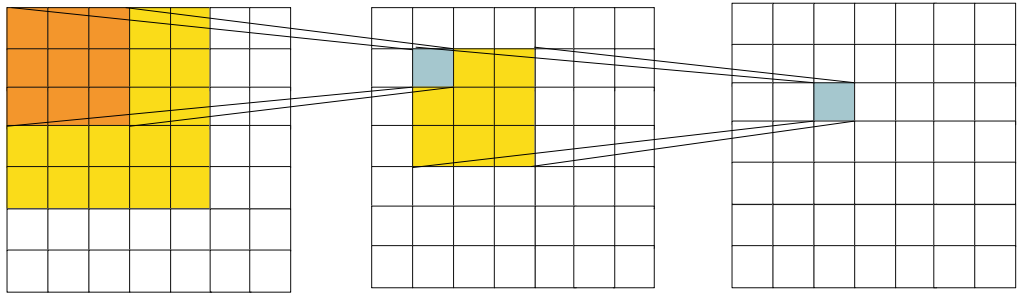
\includegraphics[width=7cm]{figure/dilatedconv-6.png}
        \caption{Receptive field of each convolution layer with a $3 \times 3$ kernel. The orange area marks the receptive field of one pixel in Layer 2, the yellow area marks the receptive field of one pixel in layer 3. } 
    \end{figure}


\begin{itemize}
        \item Intuitively, neurons in the first layers capture less information of the input (layer), while neurons in the last layers have huge receptive fields and can capture a lot more global information from the input (layer). 
        \item The size of the receptive fields depends on the filter size. 
    \end{itemize}

    \vspace*{-0.5cm}

    \begin{figure}
        \centering
        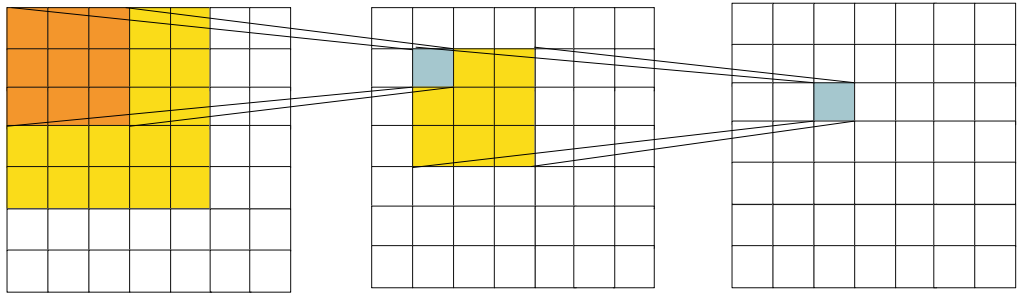
\includegraphics[width=7cm]{figure/dilatedconv-6.png}
        \caption{A convolutional neural network, convolved with $3$ layers with $3 \times 3$ kernels. The orange area marks the receptive field of one neuron in Layer 2 w.r.t. the input layer (size $9$), the yellow area marks the receptive field of one pixel in layer 3. } 
    \end{figure}

\framebreak 

\begin{itemize}
        \item By increasing the filter size, the size of the receptive fields increases as well and more contextual information can be captured.
        \item However, increasing the filter size increases the number of parameters, which leads to increased runtime. 
        \item Artificially increase the receptive field of the net without using more filter weights by adding a new dilation parameter to the kernel that skips pixels during convolution.
        \item Benefits:
        \begin{itemize}
            \item Capture more contextual information. 
            \item Enable the processing of inputs in higher dimensions to detect fine details. 
            \item Improved run-time-performance due to less parameters.
        \end{itemize}
    \end{itemize}

    \vspace*{-0.9cm}
 

\framebreak

\begin{itemize}
        \item Useful in applications where the global context is of great importance for the model decision.
        \item This component finds application in:
        \begin{itemize}
            \item Generation of audio-signals and songs within the famous Wavenet developed by DeepMind.
            \item Time series classification and forecasting.
            \item Image segmentation.
        \end{itemize}
    \end{itemize}

    \begin{figure}
        \centering
        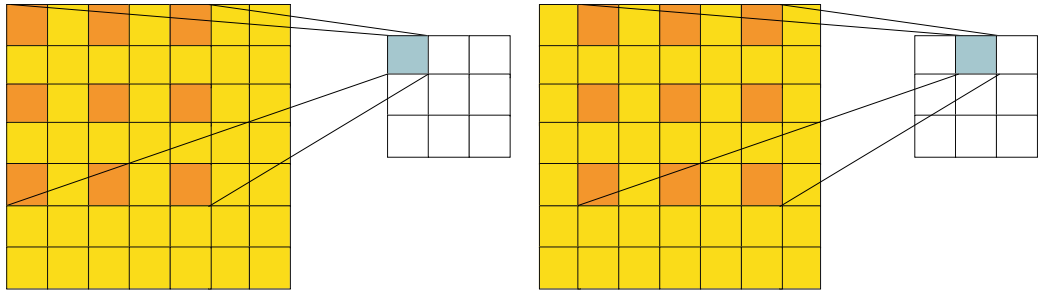
\includegraphics[width=7cm]{figure/dilatedconv-7.png}
        \caption{Dilated convolution on 2D data. A dilated kernel is a regular convolutional kernel interleaved with zeros. } 
    \end{figure}


\framebreak 

    \vspace*{0.5cm}
    \begin{figure}
        \centering
        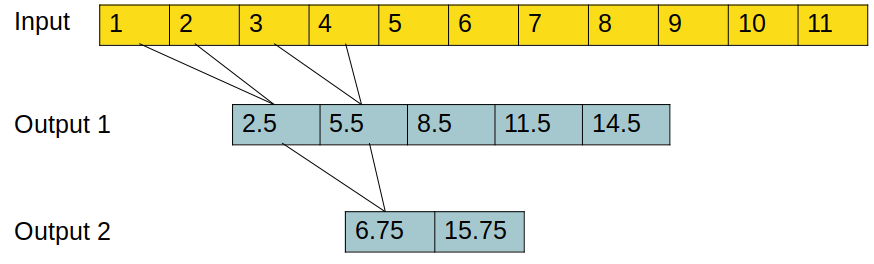
\includegraphics[width=11cm]{figure/dilatedconv-4.png}
        \caption{Simple $1$D convolutional network with convolutional kernel of size $2$, stride $2$ and fixed weights $\{0.5, 1.0\}$. \\ The kernel is not dilated (\textbf{dilation factor} $\mathbf{1}$). One neuron in layer $2$ has a receptive field of size $4$ w.r.t. the input layer. }
    \end{figure}
\framebreak 
    \vspace*{0.5cm}
    \begin{figure}
        \centering
        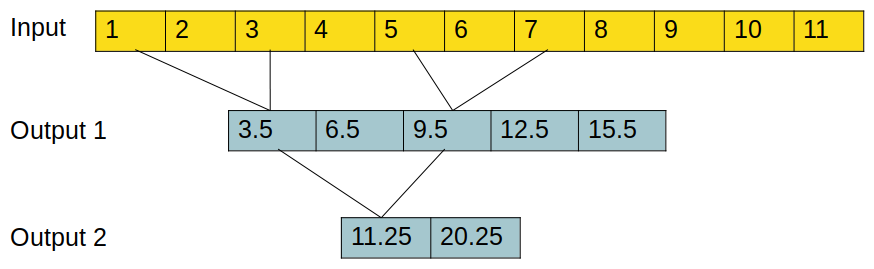
\includegraphics[width=11cm]{figure/dilatedconv-5.png}
        \caption{Simple $1$D convolutional network with convolutional kernel of size $2$, stride $2$ and fixed weights $\{0.5, 1.0\}$. \\ The kernel is dilated with \textbf{dilation factor} $\mathbf{2}$. One neuron in layer $2$ has a receptive field of size $7$ w.r.t. the input layer. }
    \end{figure}
    
\framebreak 

    \begin{figure}
        \centering
        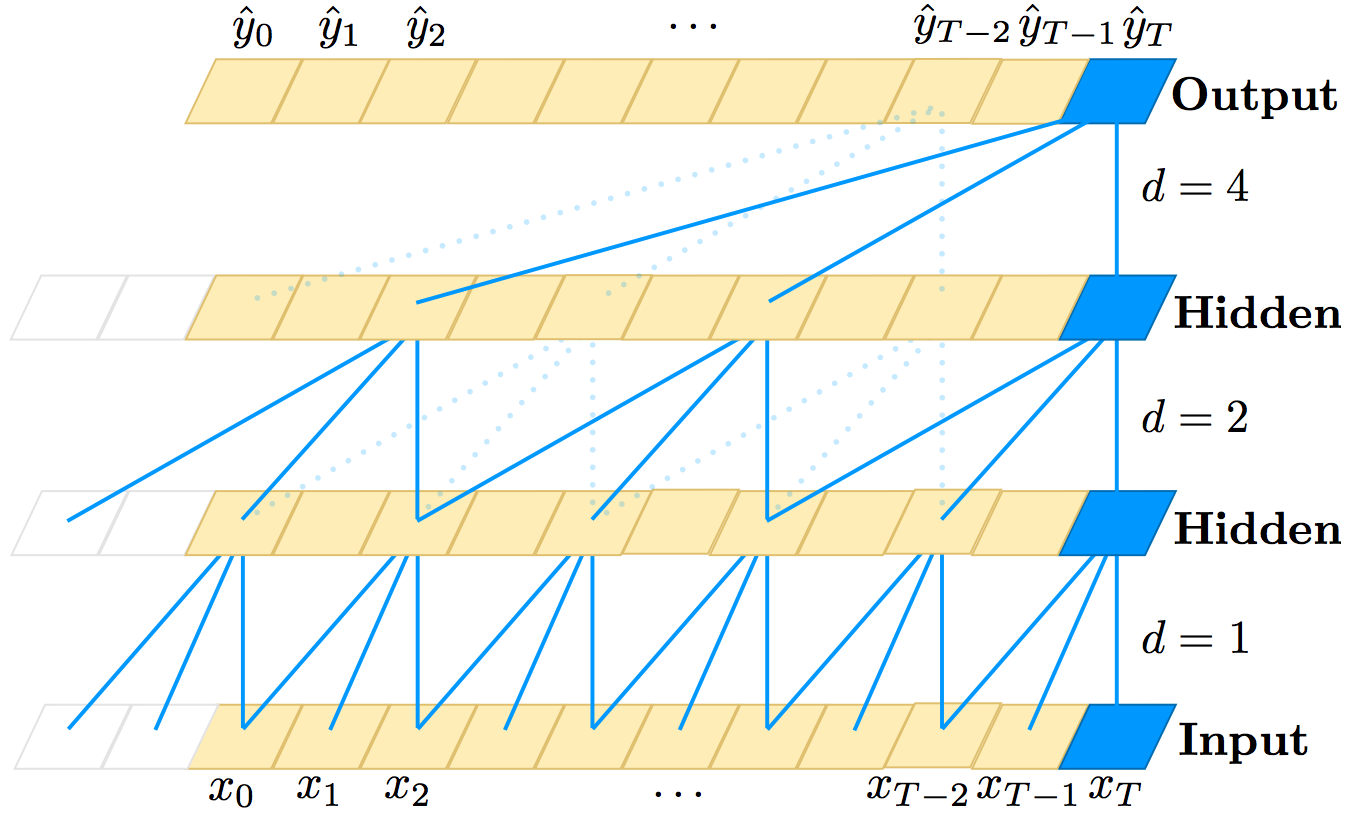
\includegraphics[width=8cm]{plots/05_conv_variations/dilated/tcn.png}
        \caption{Application of (a variant of) dilated convolutions on time series for classification or seq2seq prediction (e.g. machine translation). Given an input sequence $x_0,x_1, \ldots, x_T$, the model generates an output sequence $\yh_0,\yh_1, \ldots, \yh_T$ . Dilation factors $d = 1, 2, 4$ shown above, each with a kernel size $k = 3$. The dilations are used to drastically increase the context information for each output neuron with relatively few layers (Roy, 2019).}
    \end{figure}

\end{vbframe}
%%%%%%%%%%%%%%%%%%%%%%%%%%%%%%%%%%%%%%%%%%%%

\section{Transposed Convolutions}


\begin{vbframe}{Transposed convolutions}
    \begin{itemize}
        \item Problem setting: 
        \begin{itemize}
            \item For many applications and in many network architectures, we often want to do transformations going in the opposite direction of a normal convolution, i.e. we would like to perform up-sampling.
            \item examples include generating high-resolution images and mapping low dimensional feature map to high dimensional space such as in auto-encoder or semantic segmentation.
        \end{itemize}
        \item Instead of decreasing dimensionality as with regular convolutions, \textbf{transposed convolutions} are used to re-increase dimensionality back to the initial dimensionality.
        %\item Idea: use transposed convolutions to re-increase dimensionality instead of decreasing it as with regular convolutions.
        \item Note: Do not confuse this with deconvolutions (which are mathematically defined as the inverse of a convolution).
    \end{itemize}
    
\framebreak
\begin{itemize}
\item Example 1:
  \begin{itemize}
  \item Input: yellow feature map with dim $4\times 4$.
  \item Output: blue feature map with dim $2\times 2$.
  \end{itemize}
\end{itemize}
\begin{figure}
\centering
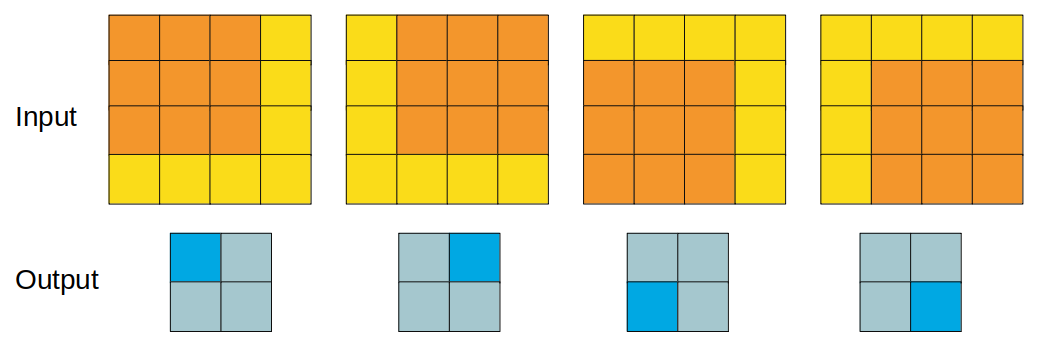
\includegraphics[width=10cm]{figure/transposedconv-1.png}
      \caption{ A \textbf{regular} convolution with kernel-size $k$ = 3, padding $p$ = 0 and stride $s$ = 1.}
\end{figure}
    Here, the feature map shrinks from $4\times 4$ to $2\times 2$.

\framebreak

%\begin{itemize}
%\item Example 1:
%        \small{
%        \begin{itemize}
%        \item Now, let us upsample the $2\times 2$ feature map %back to a $4\times 4$ feature map.
%        \item Input: $2\times 2$ (yellow). Output: $4\times 4$ %(blue).
%        \end{itemize}
\begin{itemize}
\item One way to upsample is to use a regular convolution with various padding strategies.
\end{itemize}
\begin{figure}
\centering
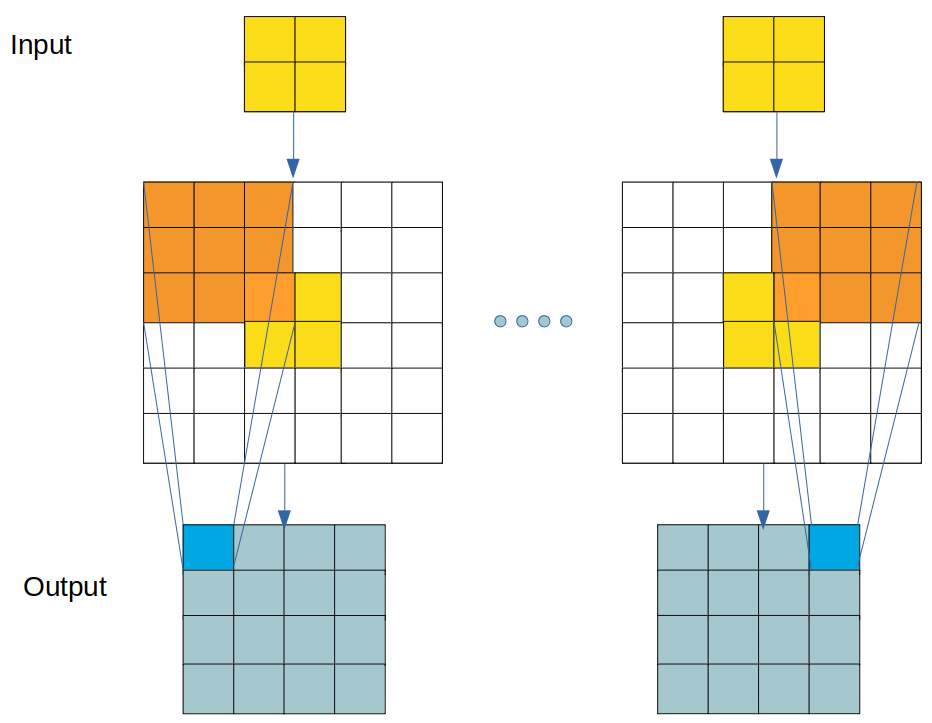
\includegraphics[width=5.5cm]{figure/transposedconv-2.png}
\caption{\textbf{Transposed} convolution can be a seen as a regular convolution. Convolution (above) with $k' = 3, s' = 1, p' = 2$ re-increases dimensionality from $2\times 2$ to $4\times 4$}
\end{figure}
    
\framebreak

\begin{itemize}
\item Convolution with parameters kernel size $k$, stride $s$ and padding factor $p$
\item Associated transposed convolution has parameters $k' = k$, $s' = s$ and $p' = k-1$
\end{itemize}

\framebreak
Example 2 : Convolution as a matrix multiplication : 
% \framebreak
%   Example 2 : Let's now view transposed convolutions from a different perspective.
\begin{figure}
\centering
\scalebox{0.75}{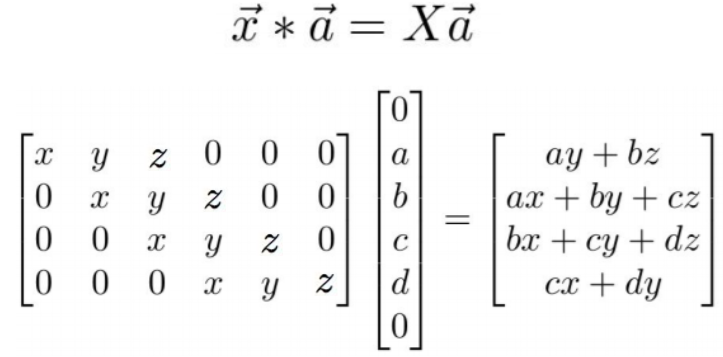
\includegraphics{plots/05_conv_variations/transpose/transpose_mat_1.png}}
\tiny{\\(Li, 2023)}
\caption{A "regular" 1D convolution. stride = 1 , padding = 1. The vector $a$ is the 1D input feature map. }
\end{figure}
   
  
\framebreak
Example 2 : Transposed Convolution as a matrix multiplication :
\begin{figure}
\centering
\scalebox{0.6}{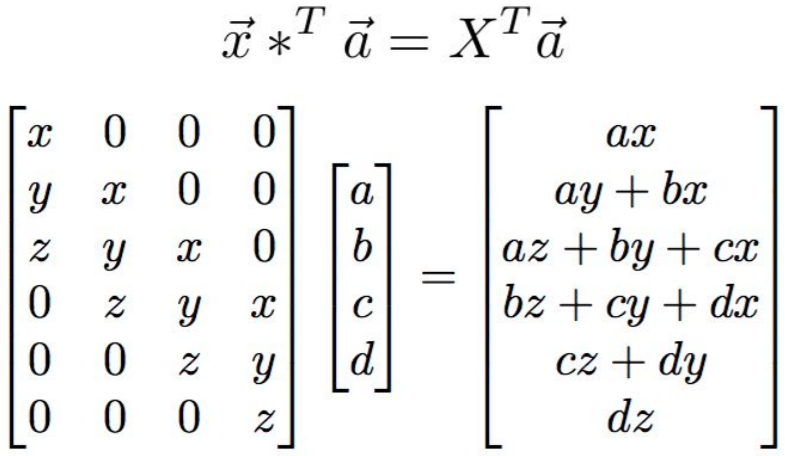
\includegraphics{plots/05_conv_variations/transpose/transpose_mat_2.png}}
\tiny{\\(Li, 2023)}
\caption{"Transposed" convolution upsamples a vector of length 4 to a vector of length 6. Stride is 1. Note the change in padding.}
\end{figure}
\small{Important : Even though the "structure" of the matrix here is the transpose of the original matrix, the non-zero elements are, in general, different from the correponding elements in the original matrix. These (non-zero) elements/weights are tuned by backpropagation.} 

\framebreak 

Example 3: Convolution as matrix multiplication:
\begin{figure}
\centering
\scalebox{0.85}{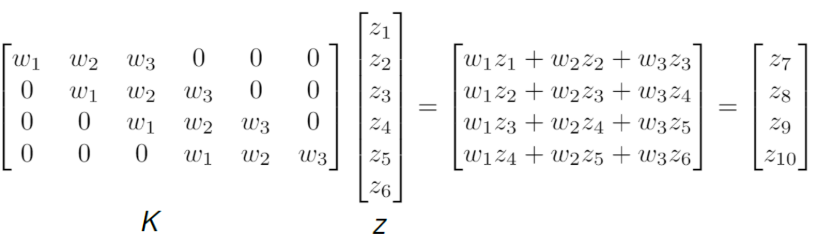
\includegraphics{plots/05_conv_variations/transpose/tr_ex21.png}}
\caption{A regular 1D convolution with  stride = 1 ,and padding = 0. The vector $z$ is in the input feature map. The matrix $K$ represents the convolution operation (Li, 2023).}
\end{figure}
  A regular convolution decreases the dimensionality of the feature map from 6 to 4.\\
\end{vbframe}
%%%%%%%%%%%%%%%%%%%%%%%%%%%%%%%%%%%%%%%%%%%%

\begin{frame}{Transposed Convolutions}

Example 3: Transposed Convolution as matrix multiplication:
\vspace*{-0.2cm}
\begin{figure}
\centering
\scalebox{0.75}{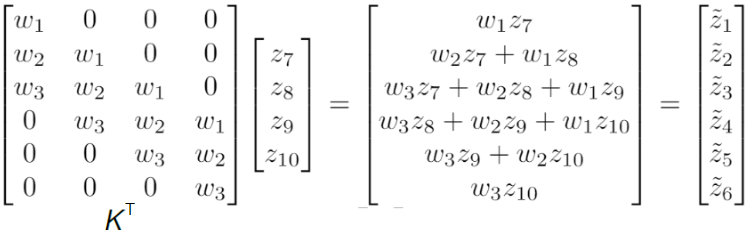
\includegraphics{plots/05_conv_variations/transpose/tr_ex22.png}}
\caption{\footnotesize{A transposed convolution can be used to upsample the feature vector of length 4 back to a feature vector of length 6 (Li, 2023).}}
\end{figure}

\vspace*{-0.4cm}

\textbf{Note}:
\begin{itemize}
  	\only<1>{\item Even though the transpose of the original matrix is shown in this example, the actual values of the weights are different from the original matrix (and optimized by backpropagation). }
  	\only<1>{\item The goal of the transposed convolution here is simply to get back the original dimensionality. It is \textit{not} necessarily to get back the original feature map itself.}
  	\only<2>{\item The elements in the downsampled vector only affect those elements in the upsampled vector that they were originally "derived" from. For example, $z_7$ was computed using $z_1$ , $z_2$ and $z_3$ and it is only used to compute $\tilde{z}_1$, $\tilde{z}_2$ and $\tilde{z}_3$.}
  	\only<2>{\item In general, transposing the original matrix does not result in a convolution. But a transposed convolution can always be implemented as a regular convolution by using various padding strategies (this would not be very efficient, however).}
\end{itemize}

\end{frame}
%%%%%%%%%%%%%%%%%%%%%%%%%%%%%%%%%%%%%%%%%%%

\begin{frame}{Transposed Convolutions}
  
  Example 4: Let us now view transposed convolutions from a different perspective.
  
  \only<1>{
  \begin{figure}
      \centering
      \scalebox{0.9}{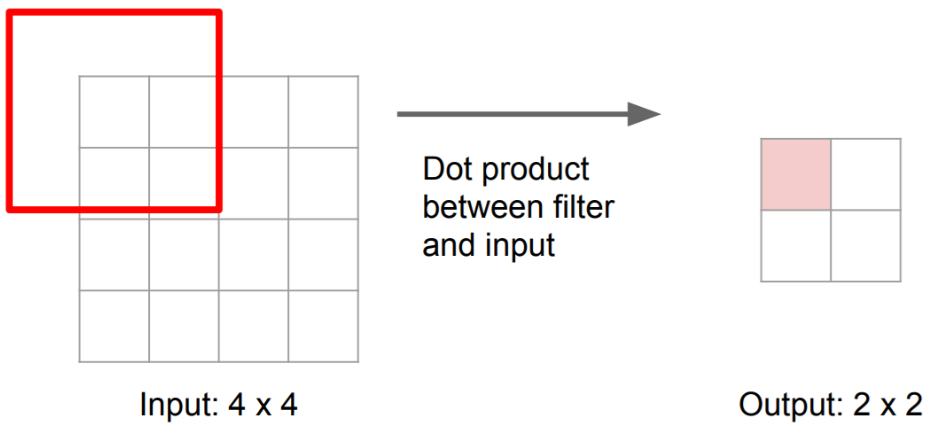
\includegraphics{plots/05_conv_variations/transpose/tr_conv_1.png}}
      \caption{Regular $3\times 3$ convolution, stride 2, padding 1 (Li, 2023).}
  \end{figure}
 }

  \only<2>{
  \begin{figure}
      \centering
      \scalebox{0.9}{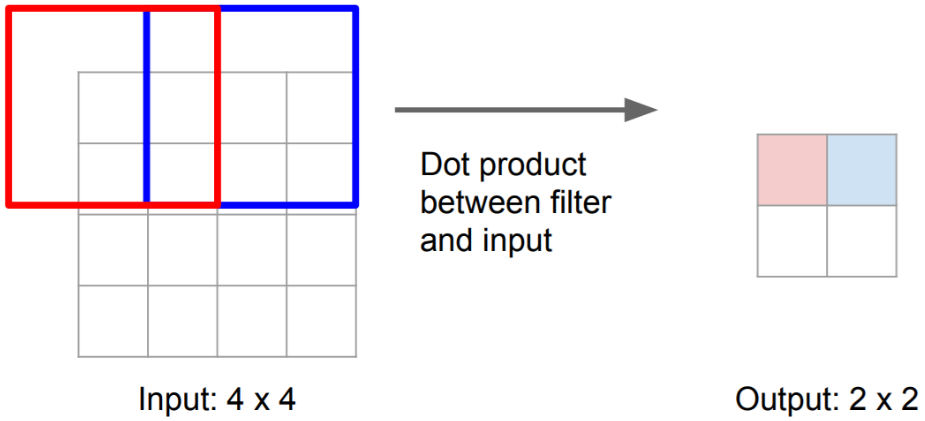
\includegraphics{plots/05_conv_variations/transpose/tr_conv_2.png}}
      \caption{Regular $3\times 3$ convolution, stride 2, padding 1 (Li, 2023).}
  \end{figure}
 }

  \only<3>{
  \begin{figure}
      \centering
      \scalebox{0.8}{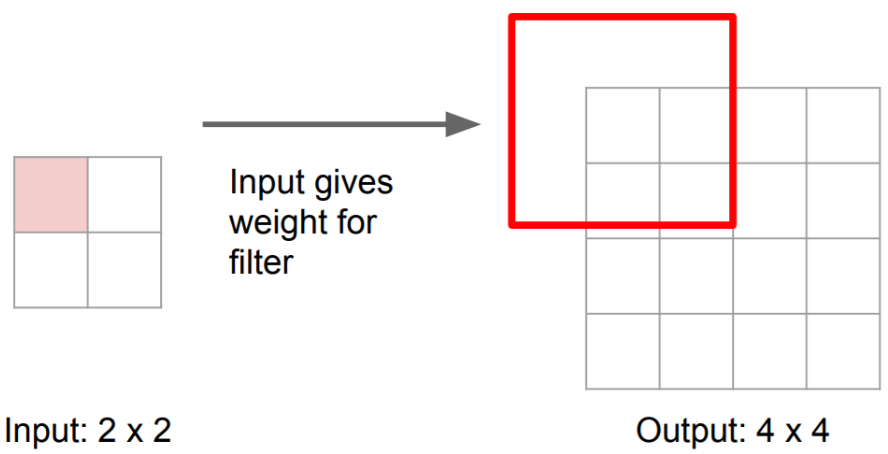
\includegraphics{plots/05_conv_variations/transpose/tr_conv_3.png}}
      \caption{\textit{Transposed} $3\times 3$ convolution, stride 2, padding 1. Note: stride now refers to the "stride" in the \textit{output} (Li, 2023).}
  \end{figure}

   Here, the filter is \textit{scaled} by the input.\\

 }

  \only<4>{
  \begin{figure}
      \centering
      \scalebox{0.8}{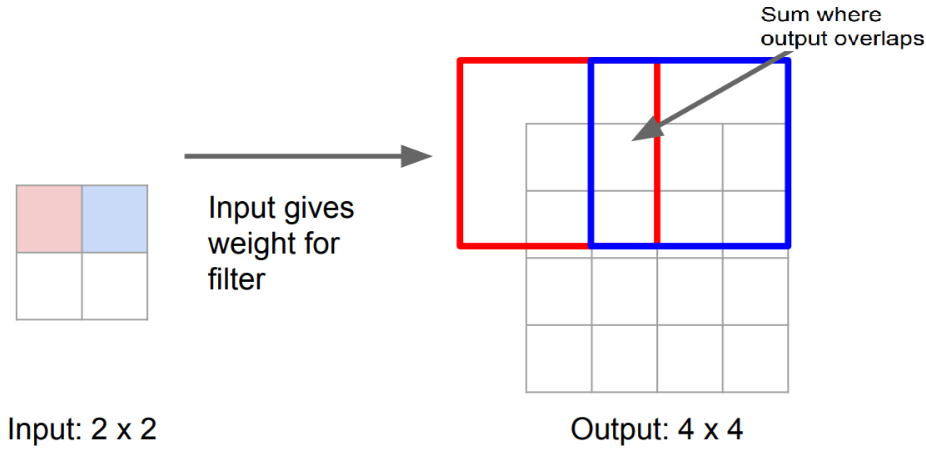
\includegraphics{plots/05_conv_variations/transpose/tr_conv_4.png}}
      \caption{\textit{Transposed} $3\times 3$ convolution, stride 2, padding 1. Note: stride now refers to the "stride" in the \textit{output} (Li, 2023).}
  \end{figure}
  Here, the filter is \textit{scaled} by the input.

 }

\end{frame}
%%%%%%%%%%%%%%%%%%%%%%%%%%%%%%%%%%%%%%

\begin{vbframe}{Transposed Convolutions -- drawback}
    \begin{figure}
        \centering
        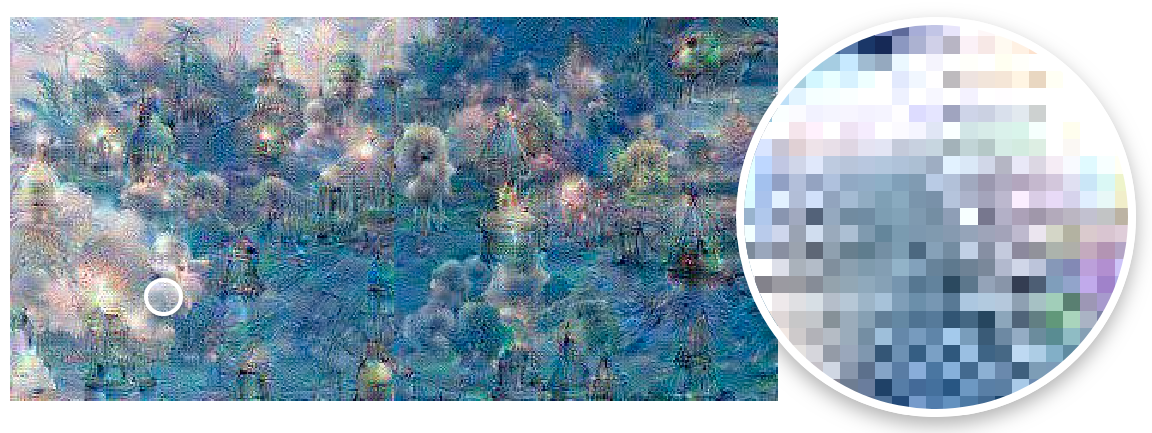
\includegraphics[width=8cm]{plots/05_conv_variations/transpose/transpose_artifact.png}
        \caption{Artifacts produced by transposed convolutions (Odena et al., 2016).}
    \end{figure}
    \begin{itemize}
        \item Transposed convolutions lead to checkerboard-style artifacts in resulting images.
    \end{itemize}
    
\framebreak

\begin{itemize}
        \small{\item Explanation: transposed convolution yields an overlap in some feature map values.
        \item This leads to higher magnitude for some feature map elements than for others, resulting in the checkerboard pattern.
        \item One solution is to ensure that the kernel size is divisible by the stride.
        }
    \end{itemize}
        \begin{figure}
            \centering
              \scalebox{0.65}{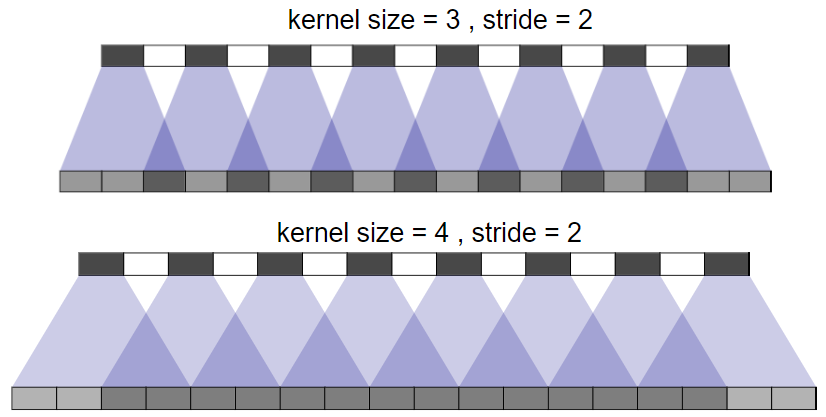
\includegraphics{plots/05_conv_variations/transpose/deconv_blog.png}}
            \caption{\footnotesize{1D example. In both images, top row = input and bottom row = output. \textit{Top}: Here, kernel weights overlap unevenly which results in a checkerboard pattern. \textit{Bottom}: There is no checkerboard pattern as the kernel size is divisible by the stride. (Odena et al., 2016)}}
        \end{figure}
       
\framebreak

\begin{itemize}
         \item Solutions: 
         \begin{itemize}
             \item Increase dimensionality via upsampling (bilinear, nearest neighbor) and then convolve this output with regular convolution.
             \item Make sure that the kernel size $k$ is divisible by the stride $s$.
         \end{itemize}
     \end{itemize}
     \begin{figure}
         \centering
         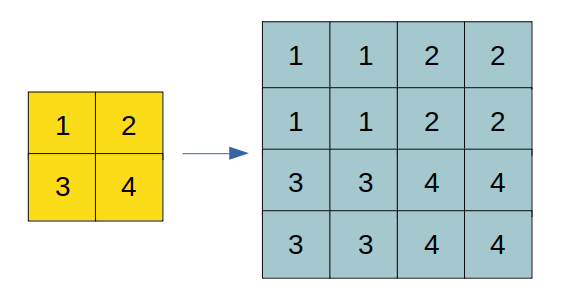
\includegraphics[width=7cm]{figure/transposedconv-last.png}
         \caption{Nearest neighbor upsampling and subsequent same convolution to avoid checkerboard patterns.}
     \end{figure}
\end{vbframe}
%%%%%%%%%%%%%%%%%%%%%%%%%%%%%%%%%%%%%%%%%%%
%%%%%%%%%%%%%%%%%%%%%%%%%%%%%%%%%%%%%%%%%%%%%%%%%%%%%%%%%%%%%%%%%%
%%%%%%%%%%%%%%%%%%%%%%%%%%%%%%%%%%%%%%%%%%%%%%%%%%%%%%%%%%%%%%%%%%
%%%%%%%%%%%%%%%%%%          REFERENCES          %%%%%%%%%%%%%%%%%%
%%%%%%%%%%%%%%%%%%%%%%%%%%%%%%%%%%%%%%%%%%%%%%%%%%%%%%%%%%%%%%%%%%
\begin{vbframe}
\frametitle{References}
\footnotesize{
\begin{thebibliography}{99}
\bibitem[(Roy, 2019)]{1} Roy, R. (2019, February 4). \textit{Temporal Convolutional Networks}. Medium. \url{https://medium.com/@raushan2807/temporal-convolutional-networks-bfea16e6d7d2}
%%%%%%%%%%%%%%%%%%%%%%%%%%%%%%%%%%%
\bibitem[(Li, 2023)]{6} Li, F.-F. (2023). \textit{Lecture 11: Detection and segmentation - Stanford University}. CS231n. \url{http://cs231n.stanford.edu/slides/2017/cs231n_2017_lecture11.pdf}
%%%%%%%%%%%%%%%%%%%%%%%%%%%%%%%%%%%
\bibitem[(Odena et al., 2016)]{3}Odena, A., Dumoulin, V., \& Olah, C. (2016, October 17). \textit{Deconvolution and checkerboard artifacts}. Distill. \url{https://distill.pub/2016/deconv-checkerboard/}



% \bibitem[Dumoulin et al., 2016]{14} Dumoulin, Vincent and Visin, Francesco (2016)
% \newblock A guide to convolution arithmetic for deep learning
% \newblock \emph{\url{https://arxiv.org/abs/1603.07285v1}}
% %%%%%%%%%%%%%%%%%%%%%%%%%%%%%%%%%%
% \bibitem[van den Oord et al., 2016]{15} Van den Oord, Aaron, Sander Dielman, Karen Simonyan, Oriol Vinyals, Alex Graves, Nal Kalchbrenner, and Koray Kavukocuoglu (2016)
% \newblock WaveNet: A Generative Model for Raw Audio
% \newblock \emph{\url{https://arxiv.org/abs/1609.03499}}
% %%%%%%%%%%%%%%%%%%%%%%%%%%%%%%%%%%
% %%%%%%%%%%%%%%%%%%%%%%%%%%%%%%%%%%
% \bibitem[Gennart et al., 1996]{17} Benoit A., Gennart, Bernard Krummenacher, Roger D. Hersch, Bernard Saugy, J.C. Hadorn and D. Mueller (1996)
% \newblock The Giga View Multiprocessor Multidisk Image Server
% \newblock \emph{\url{https://www.researchgate.net/publication/220060811_The_Giga_View_Multiprocessor_Multidisk_Image_Server}}
% %%%%%%%%%%%%%%%%%%%%%%%%%%%%%%%%%%
% %%%%%%%%%%%%%%%%%%%%%%%%%%%%%%%%%%
% \bibitem[Tran et al., 2015]{18} Tran, Du, Lubomir Bourdev, Rob Fergus,  Lorenzo Torresani and Paluri Manohar (2015)
% \newblock Learning Spatiotemporal Features with 3D Convolutional Networks
% \newblock \emph{\url{https://arxiv.org/pdf/1412.0767.pdf}}
% %%%%%%%%%%%%%%%%%%%%%%%%%%%%%%%%%%
% %%%%%%%%%%%%%%%%%%%%%%%%%%%%%%%%%%
% \bibitem[Milletari et al., 2016]{19} Milletari, Fausto, Nassir Navab and  Seyed-Ahmad Ahmadi (2016)
% \newblock V-Net: Fully Convolutional Neural Networks for
% Volumetric Medical Image Segmentation
% \newblock \emph{\url{https://arxiv.org/pdf/1606.04797.pdf}}
% %%%%%%%%%%%%%%%%%%%%%%%%%%%%%%%%%%
% %%%%%%%%%%%%%%%%%%%%%%%%%%%%%%%%%%
% \bibitem[Zhang et al., 2015]{20} Zhang, Xiang, Junbo Zhao and Yann LeCun (2015)
% \newblock Character-level Convolutional Networks for Text Classification
% \newblock \emph{\url{http://arxiv.org/abs/1509.01626}}
% %%%%%%%%%%%%%%%%%%%%%%%%%%%%%%%%%%
% %%%%%%%%%%%%%%%%%%%%%%%%%%%%%%%%%%
% \bibitem[Wang et al., 2017]{21} Wang, Zhiguang, Weizhong Yan and Tim Oates (2017)
% \newblock Time Series Classification from Scratch with Deep Neural Networks: A Strong Baseline
% \newblock \emph{\url{http://arxiv.org/abs/1509.01626}}
% %%%%%%%%%%%%%%%%%%%%%%%%%%%%%%%%%%
% %%%%%%%%%%%%%%%%%%%%%%%%%%%%%%%%%%
% \bibitem[Yu et. al, 2015]{22} Fisher Yu and Vladlen Koltun (2015)
% \newblock Multi-Scale Context Aggregation by Dilated Convolutions
% \newblock \emph{\url{https://arxiv.org/abs/1511.07122}}
% %%%%%%%%%%%%%%%%%%%%%%%%%%%%%%%%%%
% %%%%%%%%%%%%%%%%%%%%%%%%%%%%%%%%%%
% \bibitem[Bai et. al, 2018]{23} Bai, Shaojie,  Zico J. Kolter and Vladlen Koltun (2018)
% \newblock An Empirical Evaluation of Generic Convolutional and Recurrent Networks for Sequence Modeling
% \newblock \emph{\url{http://arxiv.org/abs/1509.01626}}
% %%%%%%%%%%%%%%%%%%%%%%%%%%%%%%%%%%
% %%%%%%%%%%%%%%%%%%%%%%%%%%%%%%%%%%
% \bibitem[Odena et. al , 2017]{24} Augustus Odena, Vincent Dumoulin and Chris Olah (2016)
% \newblock Deconvolution and Checkerboard Artifacts
% \newblock \emph{\url{https://distill.pub/2016/deconv-checkerboard/}{https://distill.pub/2016/deconv-checkerboard/}}
% %%%%%%%%%%%%%%%%%%%%%%%%%%%%%%%%%%
% %%%%%%%%%%%%%%%%%%%%%%%%%%%%%%%%%%
% \bibitem[Arauho et. al , 2019]{45} Andre Araujo, Wade Norris and Jack Sim (2019)
% \newblock Computing Receptive Fields of Convolutional Neural Networks
% \newblock \emph{\url{https://distill.pub/2019/computing-receptive-fields/}}
% %%%%%%%%%%%%%%%%%%%%%%%%%%%%%%%%%%
% %%%%%%%%%%%%%%%%%%%%%%%%%%%%%%%%%%
% \bibitem[Wang et. al , 2017]{31} Zhiguang Wang, Yan, Weizhong and Tim Oates (2017)
% \newblock Time series classification from scratch with deep neural networks: A
% strong baseline
% \newblock \emph{\url{https://arxiv.org/1611.06455}}
% %%%%%%%%%%%%%%%%%%%%%%%%%%%%%%%%%%
% %%%%%%%%%%%%%%%%%%%%%%%%%%%%%%%%%%
% \bibitem[Lin et al., 2017]{38} Lin, Haoning and Shi, Zhenwei and Zou, Zhengxia (2017)
% \newblock Maritime Semantic Labeling of Optical Remote Sensing Images with Multi-Scale Fully Convolutional Network

\end{thebibliography}
}
\end{vbframe}




\endlecture
\end{document}